\documentclass[10pt]{amsart}
\usepackage[margin=1.4in]{geometry}
\usepackage[usenames,dvipsnames,cmyk]{xcolor} %load first
\usepackage{cancel}
\usepackage{graphicx,subfig}
\graphicspath{ {./images/} }

\usepackage{amssymb,amsmath,enumitem,url}

\newcommand{\D}{\mathrm{d}}
\newcommand{\I}{\mathrm{i}}
\DeclareMathOperator{\sech}{sech}
% \DeclareMathOperator{\cot}{cot}
\DeclareMathOperator{\E}{e}
\DeclareMathOperator{\OO}{O}
\DeclareMathOperator{\oo}{o}
\DeclareMathOperator{\erfc}{erfc}
\DeclareMathOperator{\real}{Re}
\DeclareMathOperator{\imag}{Im}
\usepackage{tikz}
\usepackage[framemethod=tikz]{mdframed}
\theoremstyle{nonumberplain}

\mdtheorem[innertopmargin=-5pt]{sol}{Solution}
%\newmdtheoremenv[innertopmargin=-5pt]{sol}{Solution}
\definecolor{MichiganBlue}{HTML}{00274C}
\definecolor{MichiganYellow}{HTML}{FFCB05}  
\definecolor{NicePurple}{RGB}{75,56,76} %PrincePurple
\definecolor{NiceRed}{RGB}{230,37,52}
\definecolor{MidnightBlue}{rgb}{0.1, 0.1, 0.44}
\usepackage[colorlinks=true, linkcolor=MidnightBlue, citecolor=MidnightBlue, urlcolor=MidnightBlue]{hyperref}

\begin{document}
\pagestyle{empty}

\newcommand{\mline}{\vspace{.2in}\hrule\vspace{.2in}}

\noindent
\text{Hunter Lybbert} \\
\text{Student ID: 2426454} \\
\text{10-14-24} \\
\text{AMATH 567} \\

\title{\bf { Homework 3} }


\maketitle
\noindent
Collaborators*: TBD \\
\\
\tiny
\text{*Listed in no particular order. And anyone I discussed at least part of one problem with is considered a collaborator.}
\normalsize
\mline
\begin{enumerate}[label={\bf {\arabic*}:}]
\item From A\&F: 2.2.4. \\
Let $\alpha$ be a real number.
Show that the set of all values of the multivalued function $\log(z^\alpha)$ is not necessarily the same as that of $\alpha \log z$. \\
\textit{Solution:} \\
Let's begin by looking more closely at the values that the function $\alpha \log z$ can take on.
Starting with $w = \alpha \log z$, notice we have
\begin{align*}
\alpha \log z &= \alpha \log\left( r\E^{i\theta} \right) \\
		   &= \alpha \left(\log r + i\theta\right) \: \text{where we say} \:\: \theta = \theta_p + 2\pi k, \: k \in \mathbb{Z} \\
		   &= \alpha \left(\log r + i\left(\theta_p + 2\pi k\right)\right), \: k \in \mathbb{Z} \\
		   &= \alpha \left(\log r + i\theta_p + 2i\pi k \right), \: k \in \mathbb{Z} \\
		   &= \alpha \log r + \alpha i \theta_p + \alpha 2i\pi k, \: k \in \mathbb{Z}. \\
\end{align*}
Now considering the other expression
\begin{align*}
\log \left( z^\alpha \right) &= \log \left( \left(r\E^{i\theta}\right)^\alpha\right) \\
				     &= \log \left( r^\alpha \E^{i\theta\alpha}\right) \\
				     &= \log r^\alpha + i\theta\alpha  \: \text{where we say} \:\: \theta = \theta_p + 2\pi k, \: k \in \mathbb{Z} \\
				     &= \log r^\alpha + i\left(\theta_p + 2\pi k\right)\alpha  \: \text{where we say} \:\: \theta = \theta_p + 2\pi k, \: k \in \mathbb{Z} \\
				     &= \log r^\alpha + i\left(\theta_p + 2\pi k\right)\alpha, \: k \in \mathbb{Z} \\
				     &= \log r^\alpha + \alpha i \theta_p + \alpha 2i\pi k, \: k \in \mathbb{Z}. \\
\end{align*}
\item Describe the Riemann surface on which the multi-valued function
  $w(z)$, defined by $w^2=\prod_{j=1}^{n=3}\left(z-a_j\right)$ is
  single-valued. What happens for $n=4,5$ ? For $n>5$ ? You may assume
  that all the $a_j$ are distinct.\\
\textit{Solution:} \\
Let's build up to what the the Riemann surface for $w^2=\prod_{j=1}^{n=3}\left(z-a_j\right)$ will look like.
Beginning with $w^2 = z$ the branch point at the origin of the complex plane z = 0.
is moved to the location $a_0$ instead of
Reimann Surfacebe similar to that of $w^2 = z - a_0$ which is yet again similar to $w^2 = z$ except the branch point is moved to the location $a_0$ instead of the origin of the complex plane z = 0.
\item From A\&F: 2.2.5a. \\
Derive the following formulae: \\
a) $$\coth^{-1}(z) = \frac{1}{2}\log\frac{z + 1}{z - 1}$$
\textit{Solution:} \\
We begin with solving for $w$ in $z = \coth{w}$ with $w, z \in \mathbb{C}$. 
\begin{eqnarray*}
z = \coth{w} &=& \frac{\cosh w}{\sinh w} = \frac{ \frac{e^{w} + e^{-w}}{\cancel{2}} }{ \frac{e^{w} - e^{-w}}{\cancel{2}} } = \frac{ e^{w} + e^{-w} }{ e^{w} - e^{-w} } \\
	  &=& \frac{e^{w}}{e^{w}} \frac{ e^{w} + e^{-w} }{ e^{w} - e^{-w} } = \frac{ e^{2w} + 1}{ e^{2w} - 1 }
\end{eqnarray*}
Now let's proceed by multiplying both sides by the denominator
\begin{eqnarray*}
z\left( e^{2w} - 1\right) &=&  e^{2w} + 1\\
ze^{2w} - z &=&  e^{2w} + 1\\
ze^{2w} - e^{2w} &=& z + 1\\
e^{2w}(z - 1) &=& z + 1\\
e^{2w} &=& \frac{z + 1}{z - 1 }\\
\log \left(e^{2w}\right) &=& \log \left(\frac{z + 1}{z - 1} \right) + 2i\pi k, \: k \in \mathbb{Z} \\ \\
2w &=& \log \left(\frac{z + 1}{z - 1} \right) + 2i\pi k, \: k \in \mathbb{Z} \\ \\
w &=& \frac{1}{2}\log \left(\frac{z + 1}{z - 1} \right) + i\pi k, \: k \in \mathbb{Z} \\
\end{eqnarray*}
This is to show
$$\coth^{-1}(z) = \operatorname{arccot}(\coth w) = w = \frac{1}{2}\log \left(\frac{z + 1}{z - 1} \right) + i\pi k, \: k \in \mathbb{Z}.$$
More directly we have 
$$\coth^{-1}(z) = \frac{1}{2}\log \left(\frac{z + 1}{z - 1} \right) + i\pi k, \: k \in \mathbb{Z}.$$
as required. 
\textbf{TODO:} determine what your choice of $k$ should be \qed \\
b) $$\sech^{-1}(z) = \log \left(\frac{1 + (1 - z^2)^{\frac{1}{2}}}{z}\right)$$
\textit{Solution:} \\
We begin with solving for $w$ in $z = \sech{w}$ with $w, z \in \mathbb{C}$. 
\begin{eqnarray*}
z = \sech{w} &=& \frac{1}{\cosh w} = \frac{1}{\frac{e^{w} + e^{-w}}{2}} = \frac{2}{e^{w} + e^{-w}} \\
	  &=& \frac{e^{w}}{e^{w}} \frac{2}{e^{w} + e^{-w}} = \frac{ 2e^{w}}{ e^{2w} + 1 }
\end{eqnarray*}
Now let's proceed by multiplying both sides by the denominator
\begin{eqnarray*}
z\left( e^{2w} + 1 \right) &=&  2e^{w}\\
ze^{2w} + z &=&  2e^{w}\\
ze^{2w} - 2e^{w}+ z &=&  0\\
\end{eqnarray*}
We now use the quadratic formula to solve for $e^{w}$
\begin{eqnarray*}
e^{w} &=& \frac{2 + \left(4 - 4z^2\right)^{\frac{1}{2}}}{2z} \\
e^{w} &=& \frac{\cancel2 + \cancel2\left(1 - z^2\right)^{\frac{1}{2}}}{\cancel2z} \\
\log e^{w} &=& \log\left(\frac{1 + \left(1 - z^2\right)^{\frac{1}{2}}}{z} \right) + 2i\pi k, \: k \in \mathbb{Z} \\
w &=& \log\left(\frac{1 + \left(1 - z^2\right)^{\frac{1}{2}}}{z} \right) + 2i\pi k, \: k \in \mathbb{Z} \\
\end{eqnarray*}
This is to show
$$\sech^{-1}(z) = \sech^{-1}(\sech w) = w = \log\left(\frac{1 + \left(1 - z^2\right)^{\frac{1}{2}}}{z} \right) + 2i\pi k, \: k \in \mathbb{Z}.$$
More directly we have 
$$\sech^{-1}(z) = \log\left(\frac{1 + \left(1 - z^2\right)^{\frac{1}{2}}}{z} \right) + 2i\pi k, \: k \in \mathbb{Z}.$$
as required. 
\textbf{TODO:} determine what your choice of $k$ should be and how to denote the related cuts made for the $\sqrt{\cdot}$ function.
\qed \\
\\
While you're at it, also derive a formula for $\operatorname{arccot}(z)$ in terms of the logarithm. \\
\textit{Solution:} \\
Let's begin by solving for $w$ in this equation $z = \cot w$ with $w, z \in \mathbb{C}$.
\begin{eqnarray*}
z = \cot w &=& \frac{\cos w}{\sin w} = \frac{ \frac{e^{iw} + e^{-iw}}{\cancel{2}} }{ \frac{e^{iw} - e^{-iw}}{\cancel{2}i} } = \frac{ i\left(e^{iw} + e^{-iw} \right)}{ e^{iw} - e^{-iw} } \\
	  &=& \frac{e^{iw}}{e^{iw}} \frac{ i\left(e^{iw} + e^{-iw} \right)}{ e^{iw} - e^{-iw} } = \frac{ i\left(e^{2iw} + 1 \right)}{ e^{2iw} - 1 }
\end{eqnarray*}
Now let's proceed by multiplying both sides by the denominator
\begin{eqnarray*}
z(e^{2iw} - 1) &=& i\left(e^{2iw} + 1 \right) \\
ze^{2iw} - z &=& ie^{2iw} + i \\
ze^{2iw} - z - ie^{2iw} - i &=& 0 \\
e^{2iw}(z - i) &=& z + i \\ 
e^{2iw} &=& \frac{z + i}{z - i} \\
\log \left(e^{2iw}\right) &=& \log \left(\frac{z + i}{z - i} \right) + 2i\pi k, \: k \in \mathbb{Z} \\ \\
2iw &=& \log \left(\frac{z + i}{z - i} \right) + 2i\pi k, \: k \in \mathbb{Z} \\
w &=& \frac{1}{2i}\log \left(\frac{z + i}{z - i} \right) + \pi k, \: k \in \mathbb{Z} \\
\end{eqnarray*}
This is to show
$$\operatorname{arccot}(z) = \operatorname{arccot}(\cot w) = w = \frac{1}{2i}\log \left(\frac{z + i}{z - i} \right) + \pi k, \: k \in \mathbb{Z}.$$
More directly we have 
$$ \operatorname{arccot}(z) = \frac{1}{2i}\log \left(\frac{z + i}{z - i} \right) + \pi k, \: k \in \mathbb{Z}$$
as required. 
\textbf{TODO:} determine what your choice of $k$ should be \qed \\

\item Let
  \begin{align*}
    s(z) = z^{1/2} = \rho^{1/2} \E^{\I \theta/2}, \quad \theta \in [-\pi,\pi),
  \end{align*}
  denote the principal branch of the square root.  Show that the
  functions
  \begin{align*}
    f_1(z) = s(z^2 -1), \quad f_2(z) = s(z-1) s(z+1),
  \end{align*}
  are not equal as functions on $\mathbb C$ --- first produce plots and then use a mathematical argument.  Determine the branch cut for $f_2(z)$ (Note: My
  cartoon of what the branch cut for $f_1$ looks like in lecture was
  not accurate).  Find the relationship between $f_1(z)$ and $f_2(z)$.\\
\textit{Solution:} \\
\begin{figure}[h]
	\centering
	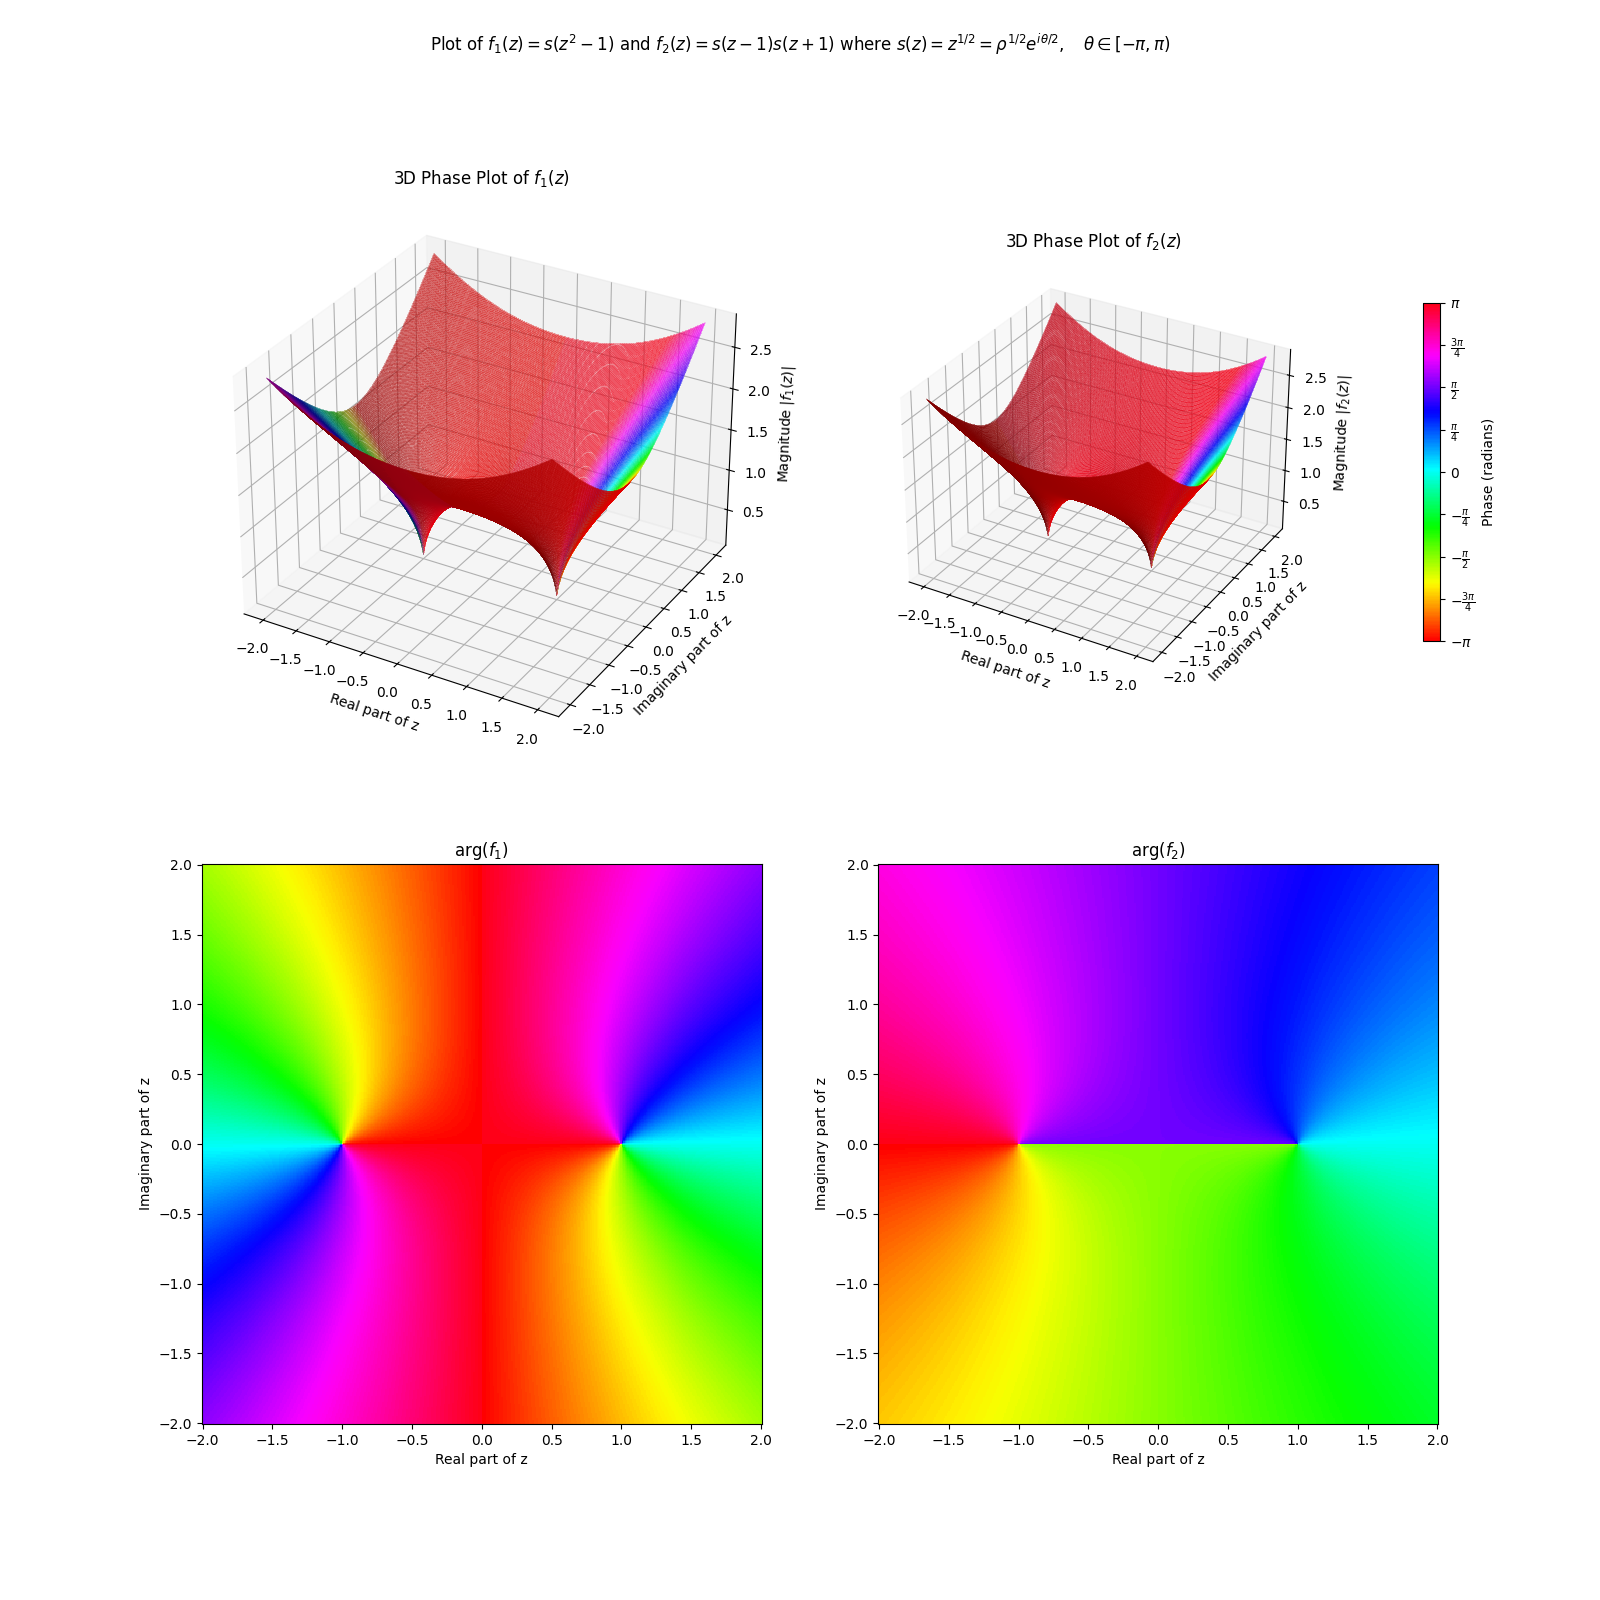
\includegraphics[width=1\textwidth]{problem_4_vis.png}
 	\caption{
	From problem 4, plot lot $f_1(z) = s(z^2 -1)$, $f_2(z) = s(z-1) s(z+1)$, where $s(z) = z^{1/2} = \rho^{1/2} \E^{\I \theta/2},\:\:
	\theta \in [-\pi,\pi)$, denote the principal branch of the square root.}\label{fig:f1}
\end{figure}
  \item Consider the function
    \begin{align*}
     \psi(z) = \int_1^z \frac{\D w}{(w^2 - 1)^{1/2}}, \quad z \not \in
      (-\infty, 1),
    \end{align*}
    where the path of integration is a straight line from $1$ to $z$.
    \begin{itemize}
   \item  Show that
    \begin{align*}
      \psi(z) = \log \varphi(z), \quad \varphi(z) = z + (z^2 -
      1)^{1/2}, \quad z \not \in
      (-\infty, 1),
    \end{align*}
   for an appropriate choice of branch cut for $(z^2 -
   1)^{1/2}$.  Here $\log z$ denotes the principal branch. \\
   \textit{Solution:} \\
   We will first show that $\log \varphi(z)$ is analytic. After which we will also show that $\log \varphi(z)$ is indeed the anti-derivative of what we have in the integrand.
   \item Find an expression for
   \begin{align*}
     \gamma(z) = \int_{-1}^z \frac{\D w}{(w^2 - 1)^{1/2}}, \quad z \not \in
      (-1, \infty),
   \end{align*}
   in terms of $\varphi(z)$ and the principal branch of the logarithm.  Again, the path of integration is a
   straight line.
 \end{itemize}
 \textit{Solution:} \\

 \item Show that $\varphi,$ from the previous problem, maps $\mathbb C \setminus [-1,1]$ onto the
   exterior of the unit disk, $\{ z \in \mathbb C ~:~ |z| > 1\}$.
   Furthermore
   \begin{align*}
     \frac 1 2 \left( \varphi(z) + 1/\varphi(z) \right) = z, \quad \mathbb C \setminus [-1,1].
   \end{align*}
\textit{Solution:} \\

   \item (Sharpness of the Bernstein--Walsh inequality)  The
     Bernstein--Walsh inequality states that if a polynomial $p_n$ of
     degree $n$ satisfies $\max_{-1 \leq x \leq 1} |p_n(x)| \leq 1$
     then
     \begin{align*}
       |p_n(z)| \leq |\varphi(z)|^n, \quad z \in \mathbb C \setminus [-1,1].
     \end{align*}
     Show that
     \begin{align*}
        T_n(z) = \frac 1 2 \left( \varphi(z)^n + \varphi(z)^{-n}
       \right), \quad z \in \mathbb C \setminus [-1,1]
     \end{align*}
     is a polynomial that satisfies
     \begin{align*}
       \max_{-1 \leq x \leq 1} |T_n(x)| &= 1,\\
       \lim_{n \to \infty} |T_n(z)|^{1/n} &= |\varphi(z)|,
     \end{align*}
     for any fixed $z \in \mathbb C \setminus [-1,1]$. \\
\textit{Solution:} \\
\end{enumerate}

\end{document}

%%% Local Variables:
%%% mode: latex
%%% TeX-master: t
%%% End:
